\documentclass[1p]{elsarticle_modified}
%\bibliographystyle{elsarticle-num}

%\usepackage[colorlinks]{hyperref}
%\usepackage{abbrmath_seonhwa} %\Abb, \Ascr, \Acal ,\Abf, \Afrak
\usepackage{amsfonts}
\usepackage{amssymb}
\usepackage{amsmath}
\usepackage{amsthm}
\usepackage{scalefnt}
\usepackage{amsbsy}
\usepackage{kotex}
\usepackage{caption}
\usepackage{subfig}
\usepackage{color}
\usepackage{graphicx}
\usepackage{xcolor} %% white, black, red, green, blue, cyan, magenta, yellow
\usepackage{float}
\usepackage{setspace}
\usepackage{hyperref}

\usepackage{tikz}
\usetikzlibrary{arrows}

\usepackage{multirow}
\usepackage{array} % fixed length table
\usepackage{hhline}

%%%%%%%%%%%%%%%%%%%%%
\makeatletter
\renewcommand*\env@matrix[1][\arraystretch]{%
	\edef\arraystretch{#1}%
	\hskip -\arraycolsep
	\let\@ifnextchar\new@ifnextchar
	\array{*\c@MaxMatrixCols c}}
\makeatother %https://tex.stackexchange.com/questions/14071/how-can-i-increase-the-line-spacing-in-a-matrix
%%%%%%%%%%%%%%%

\usepackage[normalem]{ulem}

\newcommand{\msout}[1]{\ifmmode\text{\sout{\ensuremath{#1}}}\else\sout{#1}\fi}
%SOURCE: \msout is \stkout macro in https://tex.stackexchange.com/questions/20609/strikeout-in-math-mode

\newcommand{\cancel}[1]{
	\ifmmode
	{\color{red}\msout{#1}}
	\else
	{\color{red}\sout{#1}}
	\fi
}

\newcommand{\add}[1]{
	{\color{blue}\uwave{#1}}
}

\newcommand{\replace}[2]{
	\ifmmode
	{\color{red}\msout{#1}}{\color{blue}\uwave{#2}}
	\else
	{\color{red}\sout{#1}}{\color{blue}\uwave{#2}}
	\fi
}

\newcommand{\Sol}{\mathcal{S}} %segment
\newcommand{\D}{D} %diagram
\newcommand{\A}{\mathcal{A}} %arc


%%%%%%%%%%%%%%%%%%%%%%%%%%%%%5 test

\def\sl{\operatorname{\textup{SL}}(2,\Cbb)}
\def\psl{\operatorname{\textup{PSL}}(2,\Cbb)}
\def\quan{\mkern 1mu \triangleright \mkern 1mu}

\theoremstyle{definition}
\newtheorem{thm}{Theorem}[section]
\newtheorem{prop}[thm]{Proposition}
\newtheorem{lem}[thm]{Lemma}
\newtheorem{ques}[thm]{Question}
\newtheorem{cor}[thm]{Corollary}
\newtheorem{defn}[thm]{Definition}
\newtheorem{exam}[thm]{Example}
\newtheorem{rmk}[thm]{Remark}
\newtheorem{alg}[thm]{Algorithm}

\newcommand{\I}{\sqrt{-1}}
\begin{document}

%\begin{frontmatter}
%
%\title{Boundary parabolic representations of knots up to 8 crossings}
%
%%% Group authors per affiliation:
%\author{Yunhi Cho} 
%\address{Department of Mathematics, University of Seoul, Seoul, Korea}
%\ead{yhcho@uos.ac.kr}
%
%
%\author{Seonhwa Kim} %\fnref{s_kim}}
%\address{Center for Geometry and Physics, Institute for Basic Science, Pohang, 37673, Korea}
%\ead{ryeona17@ibs.re.kr}
%
%\author{Hyuk Kim}
%\address{Department of Mathematical Sciences, Seoul National University, Seoul 08826, Korea}
%\ead{hyukkim@snu.ac.kr}
%
%\author{Seokbeom Yoon}
%\address{Department of Mathematical Sciences, Seoul National University, Seoul, 08826,  Korea}
%\ead{sbyoon15@snu.ac.kr}
%
%\begin{abstract}
%We find all boundary parabolic representation of knots up to 8 crossings.
%
%\end{abstract}
%\begin{keyword}
%    \MSC[2010] 57M25 
%\end{keyword}
%
%\end{frontmatter}

%\linenumbers
%\tableofcontents
%
\newcommand\colored[1]{\textcolor{white}{\rule[-0.35ex]{0.8em}{1.4ex}}\kern-0.8em\color{red} #1}%
%\newcommand\colored[1]{\textcolor{white}{ #1}\kern-2.17ex	\textcolor{white}{ #1}\kern-1.81ex	\textcolor{white}{ #1}\kern-2.15ex\color{red}#1	}

{\Large $\underline{11a_{295}~(K11a_{295})}$}

\setlength{\tabcolsep}{10pt}
\renewcommand{\arraystretch}{1.6}
\vspace{1cm}\begin{tabular}{m{100pt}>{\centering\arraybackslash}m{274pt}}
\multirow{5}{120pt}{
	\centering
	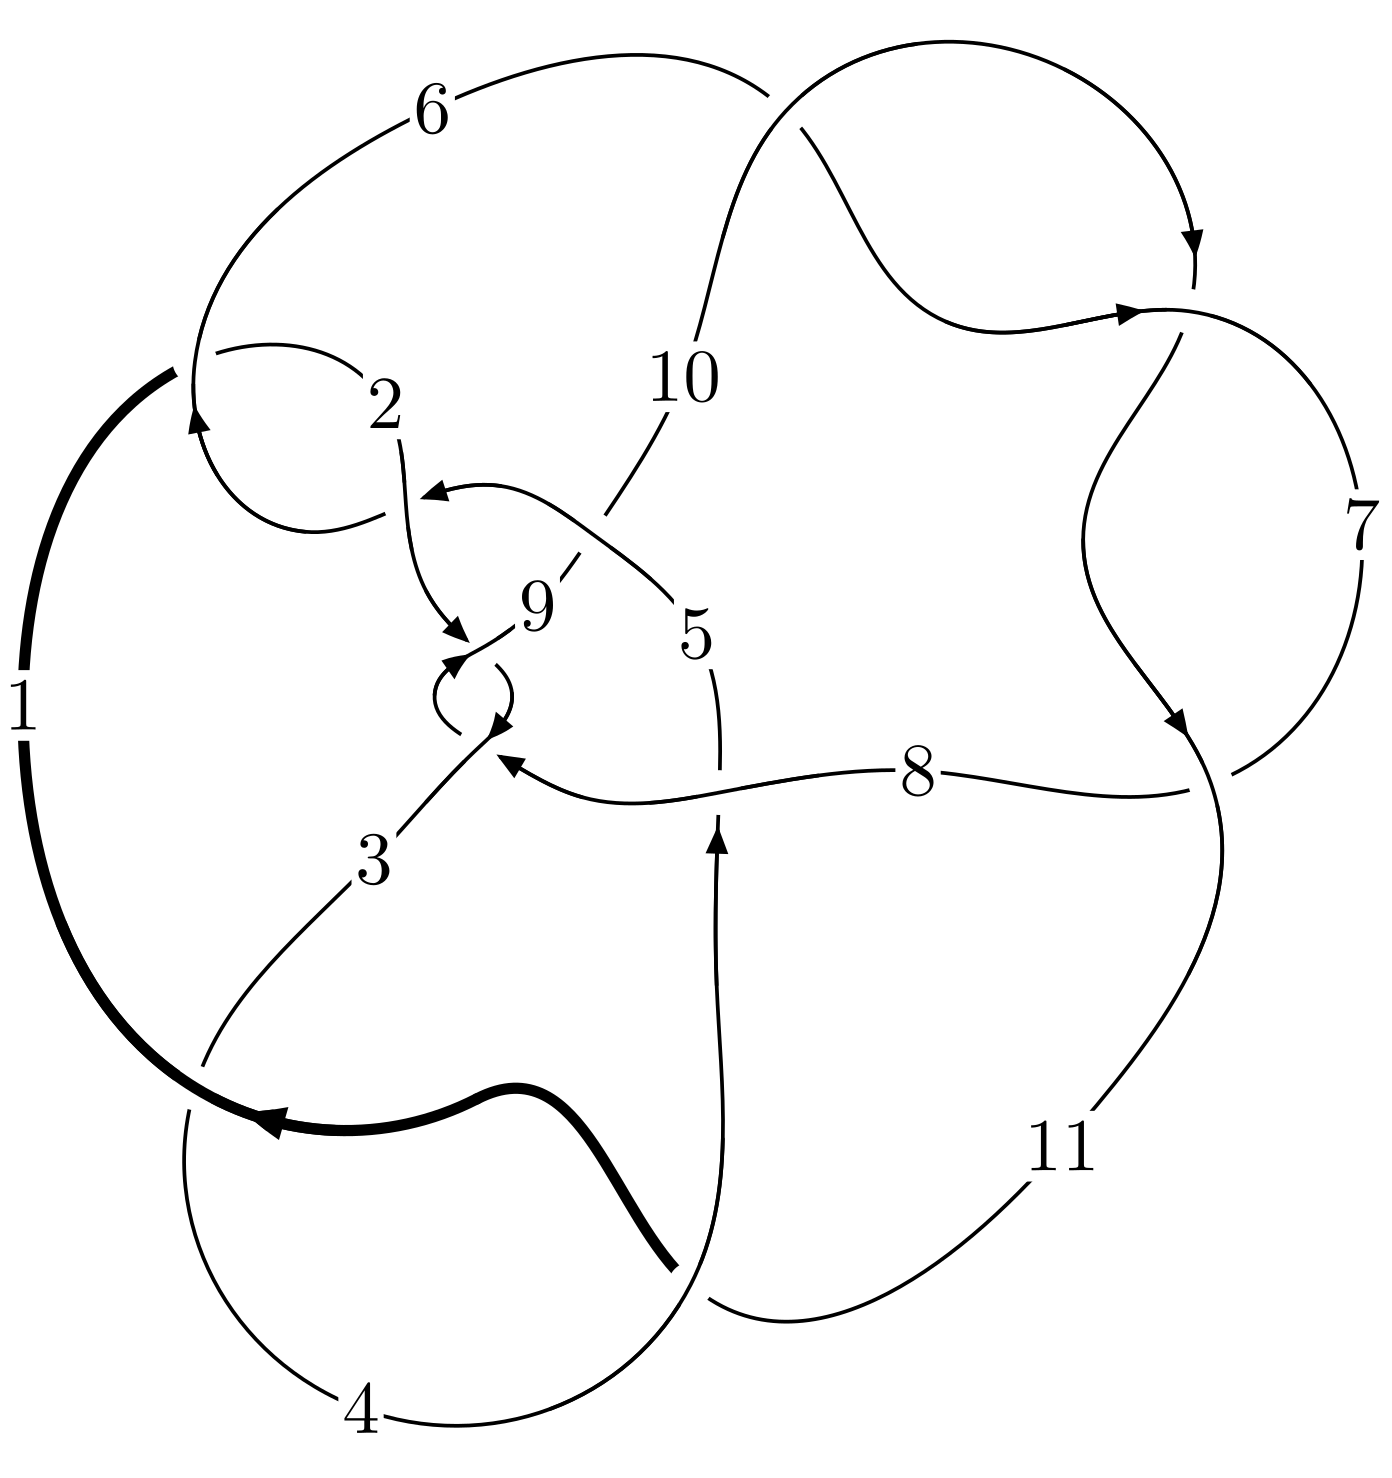
\includegraphics[width=112pt]{../../../GIT/diagram.site/Diagrams/png/544_11a_295.png}\\
\ \ \ A knot diagram\footnotemark}&
\allowdisplaybreaks
\textbf{Linearized knot diagam} \\
\cline{2-2}
 &
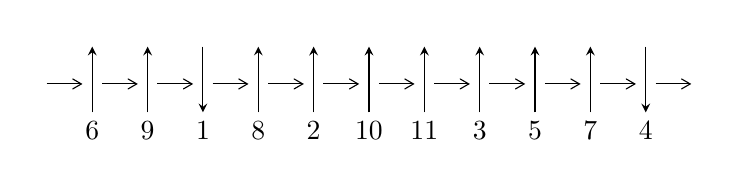
\begin{tikzpicture}[x=20pt, y=17pt]
	% nodes
	\node (C0) at (0, 0) {};
	\node (C1) at (1, 0) {};
	\node (C1U) at (1, +1) {};
	\node (C1D) at (1, -1) {6};

	\node (C2) at (2, 0) {};
	\node (C2U) at (2, +1) {};
	\node (C2D) at (2, -1) {9};

	\node (C3) at (3, 0) {};
	\node (C3U) at (3, +1) {};
	\node (C3D) at (3, -1) {1};

	\node (C4) at (4, 0) {};
	\node (C4U) at (4, +1) {};
	\node (C4D) at (4, -1) {8};

	\node (C5) at (5, 0) {};
	\node (C5U) at (5, +1) {};
	\node (C5D) at (5, -1) {2};

	\node (C6) at (6, 0) {};
	\node (C6U) at (6, +1) {};
	\node (C6D) at (6, -1) {10};

	\node (C7) at (7, 0) {};
	\node (C7U) at (7, +1) {};
	\node (C7D) at (7, -1) {11};

	\node (C8) at (8, 0) {};
	\node (C8U) at (8, +1) {};
	\node (C8D) at (8, -1) {3};

	\node (C9) at (9, 0) {};
	\node (C9U) at (9, +1) {};
	\node (C9D) at (9, -1) {5};

	\node (C10) at (10, 0) {};
	\node (C10U) at (10, +1) {};
	\node (C10D) at (10, -1) {7};

	\node (C11) at (11, 0) {};
	\node (C11U) at (11, +1) {};
	\node (C11D) at (11, -1) {4};
	\node (C12) at (12, 0) {};

	% arrows
	\draw[->,>={angle 60}]
	(C0) edge (C1) (C1) edge (C2) (C2) edge (C3) (C3) edge (C4) (C4) edge (C5) (C5) edge (C6) (C6) edge (C7) (C7) edge (C8) (C8) edge (C9) (C9) edge (C10) (C10) edge (C11) (C11) edge (C12) ;	\draw[->,>=stealth]
	(C1D) edge (C1U) (C2D) edge (C2U) (C3U) edge (C3D) (C4D) edge (C4U) (C5D) edge (C5U) (C6D) edge (C6U) (C7D) edge (C7U) (C8D) edge (C8U) (C9D) edge (C9U) (C10D) edge (C10U) (C11U) edge (C11D) ;
	\end{tikzpicture} \\
\hhline{~~} \\& 
\textbf{Solving Sequence} \\ \cline{2-2} 
 &
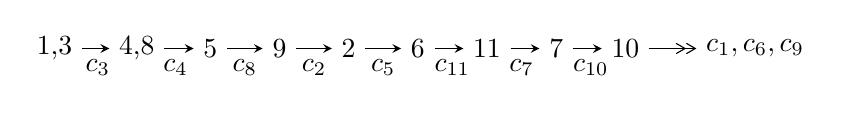
\begin{tikzpicture}[x=25pt, y=7pt]
	% node
	\node (A0) at (-1/8, 0) {1,3};
	\node (A1) at (17/16, 0) {4,8};
	\node (A2) at (17/8, 0) {5};
	\node (A3) at (25/8, 0) {9};
	\node (A4) at (33/8, 0) {2};
	\node (A5) at (41/8, 0) {6};
	\node (A6) at (49/8, 0) {11};
	\node (A7) at (57/8, 0) {7};
	\node (A8) at (65/8, 0) {10};
	\node (C1) at (1/2, -1) {$c_{3}$};
	\node (C2) at (13/8, -1) {$c_{4}$};
	\node (C3) at (21/8, -1) {$c_{8}$};
	\node (C4) at (29/8, -1) {$c_{2}$};
	\node (C5) at (37/8, -1) {$c_{5}$};
	\node (C6) at (45/8, -1) {$c_{11}$};
	\node (C7) at (53/8, -1) {$c_{7}$};
	\node (C8) at (61/8, -1) {$c_{10}$};
	\node (A9) at (10, 0) {$c_{1},c_{6},c_{9}$};

	% edge
	\draw[->,>=stealth]	
	(A0) edge (A1) (A1) edge (A2) (A2) edge (A3) (A3) edge (A4) (A4) edge (A5) (A5) edge (A6) (A6) edge (A7) (A7) edge (A8) ;
	\draw[->>,>={angle 60}]	
	(A8) edge (A9);
\end{tikzpicture} \\ 

\end{tabular} \\

\footnotetext{
The image of knot diagram is generated by the software ``\textbf{Draw programme}" developed by Andrew Bartholomew(\url{http://www.layer8.co.uk/maths/draw/index.htm\#Running-draw}), where we modified some parts for our purpose(\url{https://github.com/CATsTAILs/LinksPainter}).
}\phantom \\ \newline 
\centering \textbf{Ideals for irreducible components\footnotemark of $X_{\text{par}}$} 
 
\begin{align*}
I^u_{1}&=\langle 
1.78746\times10^{142} u^{65}-5.99607\times10^{142} u^{64}+\cdots+1.18505\times10^{143} b-1.11034\times10^{143},\\
\phantom{I^u_{1}}&\phantom{= \langle  }3.02457\times10^{142} u^{65}-1.75060\times10^{143} u^{64}+\cdots+1.54056\times10^{144} a-1.74902\times10^{145},\\
\phantom{I^u_{1}}&\phantom{= \langle  }u^{66}-3 u^{65}+\cdots+110 u+13\rangle \\
I^u_{2}&=\langle 
- u^{11}- u^{10}-4 u^9+2 u^8-2 u^7+15 u^6+5 u^5+22 u^4+3 u^3+11 u^2+b+3,\\
\phantom{I^u_{2}}&\phantom{= \langle  }- u^{11}- u^{10}-4 u^9+3 u^8+21 u^6+11 u^5+34 u^4+10 u^3+21 u^2+a+u+6,\\
\phantom{I^u_{2}}&\phantom{= \langle  }u^{12}+2 u^{11}+7 u^{10}+7 u^9+16 u^8+8 u^7+18 u^6+2 u^5+12 u^4- u^3+5 u^2- u+1\rangle \\
\\
\end{align*}
\raggedright * 2 irreducible components of $\dim_{\mathbb{C}}=0$, with total 78 representations.\\
\footnotetext{All coefficients of polynomials are rational numbers. But the coefficients are sometimes approximated in decimal forms when there is not enough margin.}
\newpage
\renewcommand{\arraystretch}{1}
\centering \section*{I. $I^u_{1}= \langle 1.79\times10^{142} u^{65}-6.00\times10^{142} u^{64}+\cdots+1.19\times10^{143} b-1.11\times10^{143},\;3.02\times10^{142} u^{65}-1.75\times10^{143} u^{64}+\cdots+1.54\times10^{144} a-1.75\times10^{145},\;u^{66}-3 u^{65}+\cdots+110 u+13 \rangle$}
\flushleft \textbf{(i) Arc colorings}\\
\begin{tabular}{m{7pt} m{180pt} m{7pt} m{180pt} }
\flushright $a_{1}=$&$\begin{pmatrix}0\\u\end{pmatrix}$ \\
\flushright $a_{3}=$&$\begin{pmatrix}1\\0\end{pmatrix}$ \\
\flushright $a_{4}=$&$\begin{pmatrix}1\\u^2\end{pmatrix}$ \\
\flushright $a_{8}=$&$\begin{pmatrix}-0.0196329 u^{65}+0.113634 u^{64}+\cdots+62.9028 u+11.3531\\-0.150834 u^{65}+0.505977 u^{64}+\cdots-0.0314640 u+0.936954\end{pmatrix}$ \\
\flushright $a_{5}=$&$\begin{pmatrix}0.224234 u^{65}-1.09610 u^{64}+\cdots-36.1801 u-11.7809\\-0.140984 u^{65}+0.152723 u^{64}+\cdots-27.9416 u-3.17071\end{pmatrix}$ \\
\flushright $a_{9}=$&$\begin{pmatrix}-0.170467 u^{65}+0.619610 u^{64}+\cdots+62.8714 u+12.2901\\-0.150834 u^{65}+0.505977 u^{64}+\cdots-0.0314640 u+0.936954\end{pmatrix}$ \\
\flushright $a_{2}=$&$\begin{pmatrix}0.199233 u^{65}-0.317764 u^{64}+\cdots+22.5218 u+12.9750\\0.0667194 u^{65}-0.184659 u^{64}+\cdots-2.86894 u-0.266940\end{pmatrix}$ \\
\flushright $a_{6}=$&$\begin{pmatrix}-0.0736024 u^{65}+0.158855 u^{64}+\cdots+67.7003 u-0.0987364\\-0.227329 u^{65}+0.752818 u^{64}+\cdots+4.04994 u+1.37421\end{pmatrix}$ \\
\flushright $a_{11}=$&$\begin{pmatrix}u\\u^3+u\end{pmatrix}$ \\
\flushright $a_{7}=$&$\begin{pmatrix}-0.194772 u^{65}+0.662394 u^{64}+\cdots+62.4963 u+11.6877\\-0.129513 u^{65}+0.444863 u^{64}+\cdots-0.728868 u+0.968066\end{pmatrix}$ \\
\flushright $a_{10}=$&$\begin{pmatrix}0.403268 u^{65}-1.30013 u^{64}+\cdots+75.9641 u+9.20323\\-0.00829394 u^{65}-0.0286337 u^{64}+\cdots-10.4471 u-0.0802321\end{pmatrix}$\\ \flushright $a_{10}=$&$\begin{pmatrix}0.403268 u^{65}-1.30013 u^{64}+\cdots+75.9641 u+9.20323\\-0.00829394 u^{65}-0.0286337 u^{64}+\cdots-10.4471 u-0.0802321\end{pmatrix}$\\&\end{tabular}
\flushleft \textbf{(ii) Obstruction class $= -1$}\\~\\
\flushleft \textbf{(iii) Cusp Shapes $= -0.295766 u^{65}+1.20445 u^{64}+\cdots+70.0120 u+13.0476$}\\~\\
\newpage\renewcommand{\arraystretch}{1}
\flushleft \textbf{(iv) u-Polynomials at the component}\newline \\
\begin{tabular}{m{50pt}|m{274pt}}
Crossings & \hspace{64pt}u-Polynomials at each crossing \\
\hline $$\begin{aligned}c_{1},c_{5}\end{aligned}$$&$\begin{aligned}
&u^{66}-2 u^{65}+\cdots-337 u+121
\end{aligned}$\\
\hline $$\begin{aligned}c_{2},c_{8}\end{aligned}$$&$\begin{aligned}
&u^{66}+u^{65}+\cdots+262 u-97
\end{aligned}$\\
\hline $$\begin{aligned}c_{3},c_{11}\end{aligned}$$&$\begin{aligned}
&u^{66}-3 u^{65}+\cdots+110 u+13
\end{aligned}$\\
\hline $$\begin{aligned}c_{4}\end{aligned}$$&$\begin{aligned}
&u^{66}-5 u^{65}+\cdots+3840 u-1447
\end{aligned}$\\
\hline $$\begin{aligned}c_{6},c_{7},c_{10}\end{aligned}$$&$\begin{aligned}
&u^{66}-5 u^{65}+\cdots-3 u-1
\end{aligned}$\\
\hline $$\begin{aligned}c_{9}\end{aligned}$$&$\begin{aligned}
&u^{66}+5 u^{64}+\cdots+2311 u-389
\end{aligned}$\\
\hline
\end{tabular}\\~\\
\newpage\renewcommand{\arraystretch}{1}
\flushleft \textbf{(v) Riley Polynomials at the component}\newline \\
\begin{tabular}{m{50pt}|m{274pt}}
Crossings & \hspace{64pt}Riley Polynomials at each crossing \\
\hline $$\begin{aligned}c_{1},c_{5}\end{aligned}$$&$\begin{aligned}
&y^{66}+42 y^{65}+\cdots+122865 y+14641
\end{aligned}$\\
\hline $$\begin{aligned}c_{2},c_{8}\end{aligned}$$&$\begin{aligned}
&y^{66}+49 y^{65}+\cdots+143204 y+9409
\end{aligned}$\\
\hline $$\begin{aligned}c_{3},c_{11}\end{aligned}$$&$\begin{aligned}
&y^{66}+47 y^{65}+\cdots-3000 y+169
\end{aligned}$\\
\hline $$\begin{aligned}c_{4}\end{aligned}$$&$\begin{aligned}
&y^{66}-19 y^{65}+\cdots-13709548 y+2093809
\end{aligned}$\\
\hline $$\begin{aligned}c_{6},c_{7},c_{10}\end{aligned}$$&$\begin{aligned}
&y^{66}-71 y^{65}+\cdots+29 y+1
\end{aligned}$\\
\hline $$\begin{aligned}c_{9}\end{aligned}$$&$\begin{aligned}
&y^{66}+10 y^{65}+\cdots+4949885 y+151321
\end{aligned}$\\
\hline
\end{tabular}\\~\\
\newpage\flushleft \textbf{(vi) Complex Volumes and Cusp Shapes}
$$\begin{array}{c|c|c}  
\text{Solutions to }I^u_{1}& \I (\text{vol} + \sqrt{-1}CS) & \text{Cusp shape}\\
 \hline 
\begin{aligned}
u &= \phantom{-}0.346412 + 0.925436 I \\
a &= -2.05986 + 0.31273 I \\
b &= -0.044674 - 1.054040 I\end{aligned}
 & -3.85841 + 0.35943 I & \phantom{-}2.42133 + 0. I\phantom{ +0.000000I} \\ \hline\begin{aligned}
u &= \phantom{-}0.346412 - 0.925436 I \\
a &= -2.05986 - 0.31273 I \\
b &= -0.044674 + 1.054040 I\end{aligned}
 & -3.85841 - 0.35943 I & \phantom{-}2.42133 + 0. I\phantom{ +0.000000I} \\ \hline\begin{aligned}
u &= \phantom{-}0.045813 + 1.027510 I \\
a &= \phantom{-}0.758381 + 1.185930 I \\
b &= -0.156972 + 1.390430 I\end{aligned}
 & \phantom{-}0.60146 - 4.40690 I & \phantom{-}7.00000 + 3.71176 I \\ \hline\begin{aligned}
u &= \phantom{-}0.045813 - 1.027510 I \\
a &= \phantom{-}0.758381 - 1.185930 I \\
b &= -0.156972 - 1.390430 I\end{aligned}
 & \phantom{-}0.60146 + 4.40690 I & \phantom{-}7.00000 - 3.71176 I \\ \hline\begin{aligned}
u &= -0.041627 + 1.032380 I \\
a &= -0.801128 + 1.092490 I \\
b &= \phantom{-}0.26921 - 1.73433 I\end{aligned}
 & \phantom{-}4.74716 + 0.24143 I & \phantom{-}11.20357 + 0. I\phantom{ +0.000000I} \\ \hline\begin{aligned}
u &= -0.041627 - 1.032380 I \\
a &= -0.801128 - 1.092490 I \\
b &= \phantom{-}0.26921 + 1.73433 I\end{aligned}
 & \phantom{-}4.74716 - 0.24143 I & \phantom{-}11.20357 + 0. I\phantom{ +0.000000I} \\ \hline\begin{aligned}
u &= -0.955497 + 0.038825 I \\
a &= \phantom{-}0.667759 - 0.483417 I \\
b &= -0.271741 - 1.131810 I\end{aligned}
 & \phantom{-}3.45574 + 3.28085 I & \phantom{-}8.60109 - 3.29735 I \\ \hline\begin{aligned}
u &= -0.955497 - 0.038825 I \\
a &= \phantom{-}0.667759 + 0.483417 I \\
b &= -0.271741 + 1.131810 I\end{aligned}
 & \phantom{-}3.45574 - 3.28085 I & \phantom{-}8.60109 + 3.29735 I \\ \hline\begin{aligned}
u &= \phantom{-}1.032800 + 0.239480 I \\
a &= -0.050681 - 0.394512 I \\
b &= -0.387740 - 1.305760 I\end{aligned}
 & -6.38275 + 5.64915 I & \phantom{-0.000000 } 0 \\ \hline\begin{aligned}
u &= \phantom{-}1.032800 - 0.239480 I \\
a &= -0.050681 + 0.394512 I \\
b &= -0.387740 + 1.305760 I\end{aligned}
 & -6.38275 - 5.64915 I & \phantom{-0.000000 } 0\\
 \hline 
 \end{array}$$\newpage$$\begin{array}{c|c|c}  
\text{Solutions to }I^u_{1}& \I (\text{vol} + \sqrt{-1}CS) & \text{Cusp shape}\\
 \hline 
\begin{aligned}
u &= \phantom{-}0.673097 + 0.824613 I \\
a &= \phantom{-}0.99902 + 1.36443 I \\
b &= -0.023131 + 1.237410 I\end{aligned}
 & -1.08058 - 2.59004 I & \phantom{-0.000000 } 0 \\ \hline\begin{aligned}
u &= \phantom{-}0.673097 - 0.824613 I \\
a &= \phantom{-}0.99902 - 1.36443 I \\
b &= -0.023131 - 1.237410 I\end{aligned}
 & -1.08058 + 2.59004 I & \phantom{-0.000000 } 0 \\ \hline\begin{aligned}
u &= \phantom{-}0.089061 + 1.093600 I \\
a &= \phantom{-}1.49100 + 0.23600 I \\
b &= -0.809871 - 0.432123 I\end{aligned}
 & \phantom{-}3.37039 - 1.11848 I & \phantom{-0.000000 } 0 \\ \hline\begin{aligned}
u &= \phantom{-}0.089061 - 1.093600 I \\
a &= \phantom{-}1.49100 - 0.23600 I \\
b &= -0.809871 + 0.432123 I\end{aligned}
 & \phantom{-}3.37039 + 1.11848 I & \phantom{-0.000000 } 0 \\ \hline\begin{aligned}
u &= \phantom{-}0.050328 + 0.893916 I \\
a &= \phantom{-}1.40705 - 2.33343 I \\
b &= \phantom{-}0.115704 + 1.020080 I\end{aligned}
 & \phantom{-}0.16047 + 3.95702 I & \phantom{-}8.80042 - 3.39843 I \\ \hline\begin{aligned}
u &= \phantom{-}0.050328 - 0.893916 I \\
a &= \phantom{-}1.40705 + 2.33343 I \\
b &= \phantom{-}0.115704 - 1.020080 I\end{aligned}
 & \phantom{-}0.16047 - 3.95702 I & \phantom{-}8.80042 + 3.39843 I \\ \hline\begin{aligned}
u &= \phantom{-}0.335391 + 1.071700 I \\
a &= \phantom{-}1.72267 - 0.57423 I \\
b &= -0.64639 + 1.48451 I\end{aligned}
 & -3.39375 - 5.20124 I & \phantom{-0.000000 } 0 \\ \hline\begin{aligned}
u &= \phantom{-}0.335391 - 1.071700 I \\
a &= \phantom{-}1.72267 + 0.57423 I \\
b &= -0.64639 - 1.48451 I\end{aligned}
 & -3.39375 + 5.20124 I & \phantom{-0.000000 } 0 \\ \hline\begin{aligned}
u &= -0.431490 + 1.050920 I \\
a &= -0.0006410 - 0.0716660 I \\
b &= \phantom{-}0.006605 + 0.382994 I\end{aligned}
 & \phantom{-}0.63556 + 2.23216 I & \phantom{-0.000000 } 0 \\ \hline\begin{aligned}
u &= -0.431490 - 1.050920 I \\
a &= -0.0006410 + 0.0716660 I \\
b &= \phantom{-}0.006605 - 0.382994 I\end{aligned}
 & \phantom{-}0.63556 - 2.23216 I & \phantom{-0.000000 } 0\\
 \hline 
 \end{array}$$\newpage$$\begin{array}{c|c|c}  
\text{Solutions to }I^u_{1}& \I (\text{vol} + \sqrt{-1}CS) & \text{Cusp shape}\\
 \hline 
\begin{aligned}
u &= -1.087080 + 0.373490 I \\
a &= -0.074311 - 0.348838 I \\
b &= \phantom{-}0.672686 - 0.122268 I\end{aligned}
 & \phantom{-}2.99874 + 4.32150 I & \phantom{-0.000000 } 0 \\ \hline\begin{aligned}
u &= -1.087080 - 0.373490 I \\
a &= -0.074311 + 0.348838 I \\
b &= \phantom{-}0.672686 + 0.122268 I\end{aligned}
 & \phantom{-}2.99874 - 4.32150 I & \phantom{-0.000000 } 0 \\ \hline\begin{aligned}
u &= \phantom{-}0.347155 + 0.753957 I \\
a &= -0.68430 - 1.36547 I \\
b &= \phantom{-}0.142627 - 1.332550 I\end{aligned}
 & -4.54149 - 3.48085 I & \phantom{-}1.46862 + 11.56926 I \\ \hline\begin{aligned}
u &= \phantom{-}0.347155 - 0.753957 I \\
a &= -0.68430 + 1.36547 I \\
b &= \phantom{-}0.142627 + 1.332550 I\end{aligned}
 & -4.54149 + 3.48085 I & \phantom{-}1.46862 - 11.56926 I \\ \hline\begin{aligned}
u &= -0.239265 + 1.179210 I \\
a &= -1.57985 + 0.23626 I \\
b &= \phantom{-}1.40483 + 0.19256 I\end{aligned}
 & \phantom{-}1.69376 + 4.59816 I & \phantom{-0.000000 } 0 \\ \hline\begin{aligned}
u &= -0.239265 - 1.179210 I \\
a &= -1.57985 - 0.23626 I \\
b &= \phantom{-}1.40483 - 0.19256 I\end{aligned}
 & \phantom{-}1.69376 - 4.59816 I & \phantom{-0.000000 } 0 \\ \hline\begin{aligned}
u &= \phantom{-}0.055605 + 1.217090 I \\
a &= \phantom{-}1.108100 + 0.672882 I \\
b &= -0.97672 - 1.47152 I\end{aligned}
 & \phantom{-}4.71138 - 2.03235 I & \phantom{-0.000000 } 0 \\ \hline\begin{aligned}
u &= \phantom{-}0.055605 - 1.217090 I \\
a &= \phantom{-}1.108100 - 0.672882 I \\
b &= -0.97672 + 1.47152 I\end{aligned}
 & \phantom{-}4.71138 + 2.03235 I & \phantom{-0.000000 } 0 \\ \hline\begin{aligned}
u &= \phantom{-}0.781623\phantom{ +0.000000I} \\
a &= \phantom{-}0.771378\phantom{ +0.000000I} \\
b &= -0.638431\phantom{ +0.000000I}\end{aligned}
 & \phantom{-}6.81634\phantom{ +0.000000I} & \phantom{-}14.5150\phantom{ +0.000000I} \\ \hline\begin{aligned}
u &= -0.748237 + 0.016944 I \\
a &= -0.293962 + 0.332817 I \\
b &= \phantom{-}0.086918 + 1.120970 I\end{aligned}
 & -2.54829 + 1.52445 I & \phantom{-}3.35567 - 4.49090 I\\
 \hline 
 \end{array}$$\newpage$$\begin{array}{c|c|c}  
\text{Solutions to }I^u_{1}& \I (\text{vol} + \sqrt{-1}CS) & \text{Cusp shape}\\
 \hline 
\begin{aligned}
u &= -0.748237 - 0.016944 I \\
a &= -0.293962 - 0.332817 I \\
b &= \phantom{-}0.086918 - 1.120970 I\end{aligned}
 & -2.54829 - 1.52445 I & \phantom{-}3.35567 + 4.49090 I \\ \hline\begin{aligned}
u &= -0.243695 + 1.234620 I \\
a &= -0.863749 - 0.292464 I \\
b &= \phantom{-}0.489851 + 0.829291 I\end{aligned}
 & \phantom{-}1.02770 + 2.29601 I & \phantom{-0.000000 } 0 \\ \hline\begin{aligned}
u &= -0.243695 - 1.234620 I \\
a &= -0.863749 + 0.292464 I \\
b &= \phantom{-}0.489851 - 0.829291 I\end{aligned}
 & \phantom{-}1.02770 - 2.29601 I & \phantom{-0.000000 } 0 \\ \hline\begin{aligned}
u &= \phantom{-}0.728717 + 1.033480 I \\
a &= \phantom{-}0.996190 + 0.473778 I \\
b &= -0.083413 + 1.085400 I\end{aligned}
 & -1.28963 - 3.11000 I & \phantom{-0.000000 } 0 \\ \hline\begin{aligned}
u &= \phantom{-}0.728717 - 1.033480 I \\
a &= \phantom{-}0.996190 - 0.473778 I \\
b &= -0.083413 - 1.085400 I\end{aligned}
 & -1.28963 + 3.11000 I & \phantom{-0.000000 } 0 \\ \hline\begin{aligned}
u &= -0.390931 + 1.215750 I \\
a &= \phantom{-}1.53205 + 0.42878 I \\
b &= -0.420123 - 1.112900 I\end{aligned}
 & \phantom{-}1.13230 + 5.61385 I & \phantom{-0.000000 } 0 \\ \hline\begin{aligned}
u &= -0.390931 - 1.215750 I \\
a &= \phantom{-}1.53205 - 0.42878 I \\
b &= -0.420123 + 1.112900 I\end{aligned}
 & \phantom{-}1.13230 - 5.61385 I & \phantom{-0.000000 } 0 \\ \hline\begin{aligned}
u &= -0.353791 + 1.249110 I \\
a &= -0.952423 - 0.041954 I \\
b &= \phantom{-}0.580495 + 0.820287 I\end{aligned}
 & \phantom{-}1.05491 + 2.33150 I & \phantom{-0.000000 } 0 \\ \hline\begin{aligned}
u &= -0.353791 - 1.249110 I \\
a &= -0.952423 + 0.041954 I \\
b &= \phantom{-}0.580495 - 0.820287 I\end{aligned}
 & \phantom{-}1.05491 - 2.33150 I & \phantom{-0.000000 } 0 \\ \hline\begin{aligned}
u &= \phantom{-}0.501327 + 0.452690 I \\
a &= \phantom{-}0.598700 - 0.082777 I \\
b &= \phantom{-}0.32459 + 1.44481 I\end{aligned}
 & -5.36608 + 1.78436 I & \phantom{-}3.12908 + 1.84447 I\\
 \hline 
 \end{array}$$\newpage$$\begin{array}{c|c|c}  
\text{Solutions to }I^u_{1}& \I (\text{vol} + \sqrt{-1}CS) & \text{Cusp shape}\\
 \hline 
\begin{aligned}
u &= \phantom{-}0.501327 - 0.452690 I \\
a &= \phantom{-}0.598700 + 0.082777 I \\
b &= \phantom{-}0.32459 - 1.44481 I\end{aligned}
 & -5.36608 - 1.78436 I & \phantom{-}3.12908 - 1.84447 I \\ \hline\begin{aligned}
u &= \phantom{-}0.365423 + 1.275750 I \\
a &= -1.277800 - 0.378899 I \\
b &= \phantom{-}0.805170 + 0.171054 I\end{aligned}
 & \phantom{-}10.80040 - 4.11654 I & \phantom{-0.000000 } 0 \\ \hline\begin{aligned}
u &= \phantom{-}0.365423 - 1.275750 I \\
a &= -1.277800 + 0.378899 I \\
b &= \phantom{-}0.805170 - 0.171054 I\end{aligned}
 & \phantom{-}10.80040 + 4.11654 I & \phantom{-0.000000 } 0 \\ \hline\begin{aligned}
u &= \phantom{-}0.541093 + 1.238690 I \\
a &= -1.53767 + 0.14911 I \\
b &= \phantom{-}0.57803 - 1.42790 I\end{aligned}
 & -3.18615 - 11.21570 I & \phantom{-0.000000 } 0 \\ \hline\begin{aligned}
u &= \phantom{-}0.541093 - 1.238690 I \\
a &= -1.53767 - 0.14911 I \\
b &= \phantom{-}0.57803 + 1.42790 I\end{aligned}
 & -3.18615 + 11.21570 I & \phantom{-0.000000 } 0 \\ \hline\begin{aligned}
u &= -0.597212 + 0.109134 I \\
a &= -0.487440 + 0.615944 I \\
b &= -0.646631 - 0.152437 I\end{aligned}
 & -2.00698 + 1.67505 I & \phantom{-}2.85750 - 4.67727 I \\ \hline\begin{aligned}
u &= -0.597212 - 0.109134 I \\
a &= -0.487440 - 0.615944 I \\
b &= -0.646631 + 0.152437 I\end{aligned}
 & -2.00698 - 1.67505 I & \phantom{-}2.85750 + 4.67727 I \\ \hline\begin{aligned}
u &= \phantom{-}1.40981 + 0.11612 I \\
a &= -0.163095 + 0.411198 I \\
b &= \phantom{-}0.430569 + 1.221430 I\end{aligned}
 & -0.32445 + 8.55031 I & \phantom{-0.000000 } 0 \\ \hline\begin{aligned}
u &= \phantom{-}1.40981 - 0.11612 I \\
a &= -0.163095 - 0.411198 I \\
b &= \phantom{-}0.430569 - 1.221430 I\end{aligned}
 & -0.32445 - 8.55031 I & \phantom{-0.000000 } 0 \\ \hline\begin{aligned}
u &= -0.51734 + 1.31863 I \\
a &= -1.62787 - 0.07441 I \\
b &= \phantom{-}0.418270 + 1.216760 I\end{aligned}
 & \phantom{-}7.53925 + 8.57953 I & \phantom{-0.000000 } 0\\
 \hline 
 \end{array}$$\newpage$$\begin{array}{c|c|c}  
\text{Solutions to }I^u_{1}& \I (\text{vol} + \sqrt{-1}CS) & \text{Cusp shape}\\
 \hline 
\begin{aligned}
u &= -0.51734 - 1.31863 I \\
a &= -1.62787 + 0.07441 I \\
b &= \phantom{-}0.418270 - 1.216760 I\end{aligned}
 & \phantom{-}7.53925 - 8.57953 I & \phantom{-0.000000 } 0 \\ \hline\begin{aligned}
u &= -0.39858 + 1.41998 I \\
a &= \phantom{-}1.206100 - 0.227250 I \\
b &= -1.212910 - 0.088188 I\end{aligned}
 & \phantom{-}8.62445 + 9.32694 I & \phantom{-0.000000 } 0 \\ \hline\begin{aligned}
u &= -0.39858 - 1.41998 I \\
a &= \phantom{-}1.206100 + 0.227250 I \\
b &= -1.212910 + 0.088188 I\end{aligned}
 & \phantom{-}8.62445 - 9.32694 I & \phantom{-0.000000 } 0 \\ \hline\begin{aligned}
u &= \phantom{-}0.16422 + 1.53291 I \\
a &= \phantom{-}0.599718 - 0.042213 I \\
b &= -0.669641 - 0.580855 I\end{aligned}
 & \phantom{-}6.78842 + 2.02734 I & \phantom{-0.000000 } 0 \\ \hline\begin{aligned}
u &= \phantom{-}0.16422 - 1.53291 I \\
a &= \phantom{-}0.599718 + 0.042213 I \\
b &= -0.669641 + 0.580855 I\end{aligned}
 & \phantom{-}6.78842 - 2.02734 I & \phantom{-0.000000 } 0 \\ \hline\begin{aligned}
u &= \phantom{-}0.63083 + 1.41800 I \\
a &= \phantom{-}1.348130 - 0.018048 I \\
b &= -0.55812 + 1.41815 I\end{aligned}
 & \phantom{-}3.9251 - 15.5092 I & \phantom{-0.000000 } 0 \\ \hline\begin{aligned}
u &= \phantom{-}0.63083 - 1.41800 I \\
a &= \phantom{-}1.348130 + 0.018048 I \\
b &= -0.55812 - 1.41815 I\end{aligned}
 & \phantom{-}3.9251 + 15.5092 I & \phantom{-0.000000 } 0 \\ \hline\begin{aligned}
u &= -0.50208 + 1.52607 I \\
a &= -0.240163 + 0.136220 I \\
b &= \phantom{-}0.200360 - 0.695523 I\end{aligned}
 & \phantom{-}7.42737 + 2.83943 I & \phantom{-0.000000 } 0 \\ \hline\begin{aligned}
u &= -0.50208 - 1.52607 I \\
a &= -0.240163 - 0.136220 I \\
b &= \phantom{-}0.200360 + 0.695523 I\end{aligned}
 & \phantom{-}7.42737 - 2.83943 I & \phantom{-0.000000 } 0 \\ \hline\begin{aligned}
u &= -0.74136 + 1.51980 I \\
a &= \phantom{-}0.786039 - 0.184606 I \\
b &= -0.662180 - 0.862296 I\end{aligned}
 & \phantom{-}6.10476 + 3.03885 I & \phantom{-0.000000 } 0\\
 \hline 
 \end{array}$$\newpage$$\begin{array}{c|c|c}  
\text{Solutions to }I^u_{1}& \I (\text{vol} + \sqrt{-1}CS) & \text{Cusp shape}\\
 \hline 
\begin{aligned}
u &= -0.74136 - 1.51980 I \\
a &= \phantom{-}0.786039 + 0.184606 I \\
b &= -0.662180 + 0.862296 I\end{aligned}
 & \phantom{-}6.10476 - 3.03885 I & \phantom{-0.000000 } 0 \\ \hline\begin{aligned}
u &= \phantom{-}1.01838 + 1.36708 I \\
a &= -0.624946 - 0.274570 I \\
b &= \phantom{-}0.141222 - 1.012850 I\end{aligned}
 & \phantom{-}6.59255 - 4.44136 I & \phantom{-0.000000 } 0 \\ \hline\begin{aligned}
u &= \phantom{-}1.01838 - 1.36708 I \\
a &= -0.624946 + 0.274570 I \\
b &= \phantom{-}0.141222 + 1.012850 I\end{aligned}
 & \phantom{-}6.59255 + 4.44136 I & \phantom{-0.000000 } 0 \\ \hline\begin{aligned}
u &= \phantom{-}0.185031\phantom{ +0.000000I} \\
a &= -1.77117\phantom{ +0.000000I} \\
b &= \phantom{-}0.368557\phantom{ +0.000000I}\end{aligned}
 & \phantom{-}0.660290\phantom{ +0.000000I} & \phantom{-}15.1130\phantom{ +0.000000I} \\ \hline\begin{aligned}
u &= -0.0705906 + 0.0713114 I \\
a &= \phantom{-}6.94504 + 10.19820 I \\
b &= \phantom{-}0.538056 - 0.549223 I\end{aligned}
 & \phantom{-}1.13118 + 1.76995 I & \phantom{-}5.98304 + 2.62479 I \\ \hline\begin{aligned}
u &= -0.0705906 - 0.0713114 I \\
a &= \phantom{-}6.94504 - 10.19820 I \\
b &= \phantom{-}0.538056 + 0.549223 I\end{aligned}
 & \phantom{-}1.13118 - 1.76995 I & \phantom{-}5.98304 - 2.62479 I\\
 \hline 
 \end{array}$$\newpage\newpage\renewcommand{\arraystretch}{1}
\centering \section*{II. $I^u_{2}= \langle - u^{11}- u^{10}+\cdots+b+3,\;- u^{11}- u^{10}+\cdots+a+6,\;u^{12}+2 u^{11}+\cdots- u+1 \rangle$}
\flushleft \textbf{(i) Arc colorings}\\
\begin{tabular}{m{7pt} m{180pt} m{7pt} m{180pt} }
\flushright $a_{1}=$&$\begin{pmatrix}0\\u\end{pmatrix}$ \\
\flushright $a_{3}=$&$\begin{pmatrix}1\\0\end{pmatrix}$ \\
\flushright $a_{4}=$&$\begin{pmatrix}1\\u^2\end{pmatrix}$ \\
\flushright $a_{8}=$&$\begin{pmatrix}u^{11}+u^{10}+4 u^9-3 u^8-21 u^6-11 u^5-34 u^4-10 u^3-21 u^2- u-6\\u^{11}+u^{10}+4 u^9-2 u^8+2 u^7-15 u^6-5 u^5-22 u^4-3 u^3-11 u^2-3\end{pmatrix}$ \\
\flushright $a_{5}=$&$\begin{pmatrix}-7 u^{11}-17 u^{10}+\cdots-18 u+3\\- u^{11}-2 u^{10}+\cdots-4 u+2\end{pmatrix}$ \\
\flushright $a_{9}=$&$\begin{pmatrix}2 u^{11}+2 u^{10}+\cdots- u-9\\u^{11}+u^{10}+4 u^9-2 u^8+2 u^7-15 u^6-5 u^5-22 u^4-3 u^3-11 u^2-3\end{pmatrix}$ \\
\flushright $a_{2}=$&$\begin{pmatrix}4 u^{11}+7 u^{10}+\cdots+9 u-8\\- u^{10}-2 u^9-6 u^8-5 u^7-10 u^6-3 u^5-8 u^4+u^3-4 u^2-2\end{pmatrix}$ \\
\flushright $a_{6}=$&$\begin{pmatrix}u^{11}+3 u^{10}+\cdots+4 u+4\\u^{11}+2 u^{10}+6 u^9+5 u^8+10 u^7+3 u^6+8 u^5- u^4+4 u^3+u^2+2 u\end{pmatrix}$ \\
\flushright $a_{11}=$&$\begin{pmatrix}u\\u^3+u\end{pmatrix}$ \\
\flushright $a_{7}=$&$\begin{pmatrix}u^{11}+u^{10}+4 u^9-3 u^8-21 u^6-11 u^5-33 u^4-9 u^3-19 u^2- u-5\\u^{11}+u^{10}+4 u^9-2 u^8+2 u^7-14 u^6-4 u^5-19 u^4-2 u^3-8 u^2-2\end{pmatrix}$ \\
\flushright $a_{10}=$&$\begin{pmatrix}- u^{11}- u^9+\cdots+5 u+6\\u^{11}+3 u^{10}+\cdots+3 u+2\end{pmatrix}$\\ \flushright $a_{10}=$&$\begin{pmatrix}- u^{11}- u^9+\cdots+5 u+6\\u^{11}+3 u^{10}+\cdots+3 u+2\end{pmatrix}$\\&\end{tabular}
\flushleft \textbf{(ii) Obstruction class $= 1$}\\~\\
\flushleft \textbf{(iii) Cusp Shapes $= 4 u^{11}+11 u^{10}+35 u^9+50 u^8+91 u^7+84 u^6+111 u^5+63 u^4+65 u^3+24 u^2+15 u+13$}\\~\\
\newpage\renewcommand{\arraystretch}{1}
\flushleft \textbf{(iv) u-Polynomials at the component}\newline \\
\begin{tabular}{m{50pt}|m{274pt}}
Crossings & \hspace{64pt}u-Polynomials at each crossing \\
\hline $$\begin{aligned}c_{1}\end{aligned}$$&$\begin{aligned}
&u^{12}- u^{11}+\cdots+2 u+1
\end{aligned}$\\
\hline $$\begin{aligned}c_{2}\end{aligned}$$&$\begin{aligned}
&u^{12}+6 u^{10}+\cdots-3 u+1
\end{aligned}$\\
\hline $$\begin{aligned}c_{3}\end{aligned}$$&$\begin{aligned}
&u^{12}+2 u^{11}+\cdots- u+1
\end{aligned}$\\
\hline $$\begin{aligned}c_{4}\end{aligned}$$&$\begin{aligned}
&u^{12}+2 u^{10}-3 u^9+7 u^8-6 u^6+8 u^5+7 u^4-2 u^3+u^2+3 u+1
\end{aligned}$\\
\hline $$\begin{aligned}c_{5}\end{aligned}$$&$\begin{aligned}
&u^{12}+u^{11}+\cdots-2 u+1
\end{aligned}$\\
\hline $$\begin{aligned}c_{6},c_{7}\end{aligned}$$&$\begin{aligned}
&u^{12}-8 u^{10}+24 u^8-32 u^6- u^5+18 u^4+u^3-3 u^2+1
\end{aligned}$\\
\hline $$\begin{aligned}c_{8}\end{aligned}$$&$\begin{aligned}
&u^{12}+6 u^{10}+\cdots+3 u+1
\end{aligned}$\\
\hline $$\begin{aligned}c_{9}\end{aligned}$$&$\begin{aligned}
&u^{12}+u^{11}- u^{10}+7 u^8-8 u^7+7 u^6-5 u^5+10 u^4-10 u^3+7 u^2-2 u+1
\end{aligned}$\\
\hline $$\begin{aligned}c_{10}\end{aligned}$$&$\begin{aligned}
&u^{12}-8 u^{10}+24 u^8-32 u^6+u^5+18 u^4- u^3-3 u^2+1
\end{aligned}$\\
\hline $$\begin{aligned}c_{11}\end{aligned}$$&$\begin{aligned}
&u^{12}-2 u^{11}+\cdots+u+1
\end{aligned}$\\
\hline
\end{tabular}\\~\\
\newpage\renewcommand{\arraystretch}{1}
\flushleft \textbf{(v) Riley Polynomials at the component}\newline \\
\begin{tabular}{m{50pt}|m{274pt}}
Crossings & \hspace{64pt}Riley Polynomials at each crossing \\
\hline $$\begin{aligned}c_{1},c_{5}\end{aligned}$$&$\begin{aligned}
&y^{12}+9 y^{11}+\cdots+10 y+1
\end{aligned}$\\
\hline $$\begin{aligned}c_{2},c_{8}\end{aligned}$$&$\begin{aligned}
&y^{12}+12 y^{11}+\cdots+5 y+1
\end{aligned}$\\
\hline $$\begin{aligned}c_{3},c_{11}\end{aligned}$$&$\begin{aligned}
&y^{12}+10 y^{11}+\cdots+9 y+1
\end{aligned}$\\
\hline $$\begin{aligned}c_{4}\end{aligned}$$&$\begin{aligned}
&y^{12}+4 y^{11}+\cdots-7 y+1
\end{aligned}$\\
\hline $$\begin{aligned}c_{6},c_{7},c_{10}\end{aligned}$$&$\begin{aligned}
&y^{12}-16 y^{11}+\cdots-6 y+1
\end{aligned}$\\
\hline $$\begin{aligned}c_{9}\end{aligned}$$&$\begin{aligned}
&y^{12}-3 y^{11}+\cdots+10 y+1
\end{aligned}$\\
\hline
\end{tabular}\\~\\
\newpage\flushleft \textbf{(vi) Complex Volumes and Cusp Shapes}
$$\begin{array}{c|c|c}  
\text{Solutions to }I^u_{2}& \I (\text{vol} + \sqrt{-1}CS) & \text{Cusp shape}\\
 \hline 
\begin{aligned}
u &= -0.369646 + 0.777513 I \\
a &= -0.17021 + 1.45709 I \\
b &= \phantom{-}0.436264 - 0.375928 I\end{aligned}
 & \phantom{-}1.64985 + 2.57365 I & \phantom{-}12.02620 - 3.39540 I \\ \hline\begin{aligned}
u &= -0.369646 - 0.777513 I \\
a &= -0.17021 - 1.45709 I \\
b &= \phantom{-}0.436264 + 0.375928 I\end{aligned}
 & \phantom{-}1.64985 - 2.57365 I & \phantom{-}12.02620 + 3.39540 I \\ \hline\begin{aligned}
u &= \phantom{-}0.149040 + 1.211350 I \\
a &= \phantom{-}0.533757 + 0.789884 I \\
b &= -0.57539 - 1.56859 I\end{aligned}
 & \phantom{-}5.02229 - 1.34240 I & \phantom{-}13.23433 + 1.17063 I \\ \hline\begin{aligned}
u &= \phantom{-}0.149040 - 1.211350 I \\
a &= \phantom{-}0.533757 - 0.789884 I \\
b &= -0.57539 + 1.56859 I\end{aligned}
 & \phantom{-}5.02229 + 1.34240 I & \phantom{-}13.23433 - 1.17063 I \\ \hline\begin{aligned}
u &= \phantom{-}0.286338 + 0.674056 I \\
a &= \phantom{-}1.23982 + 0.95839 I \\
b &= -0.211327 + 1.361950 I\end{aligned}
 & -4.35770 - 2.95981 I & \phantom{-}6.70212 - 1.32008 I \\ \hline\begin{aligned}
u &= \phantom{-}0.286338 - 0.674056 I \\
a &= \phantom{-}1.23982 - 0.95839 I \\
b &= -0.211327 - 1.361950 I\end{aligned}
 & -4.35770 + 2.95981 I & \phantom{-}6.70212 + 1.32008 I \\ \hline\begin{aligned}
u &= -0.512766 + 1.211820 I \\
a &= -0.805948 + 0.152900 I \\
b &= \phantom{-}0.476182 + 0.586558 I\end{aligned}
 & \phantom{-}0.99987 + 2.95882 I & \phantom{-}8.95384 - 10.28538 I \\ \hline\begin{aligned}
u &= -0.512766 - 1.211820 I \\
a &= -0.805948 - 0.152900 I \\
b &= \phantom{-}0.476182 - 0.586558 I\end{aligned}
 & \phantom{-}0.99987 - 2.95882 I & \phantom{-}8.95384 + 10.28538 I \\ \hline\begin{aligned}
u &= \phantom{-}0.321964 + 0.480875 I \\
a &= \phantom{-}0.07177 - 3.69908 I \\
b &= \phantom{-}0.151135 - 1.234650 I\end{aligned}
 & -1.09062 - 4.53454 I & \phantom{-}3.08537 + 5.69650 I \\ \hline\begin{aligned}
u &= \phantom{-}0.321964 - 0.480875 I \\
a &= \phantom{-}0.07177 + 3.69908 I \\
b &= \phantom{-}0.151135 + 1.234650 I\end{aligned}
 & -1.09062 + 4.53454 I & \phantom{-}3.08537 - 5.69650 I\\
 \hline 
 \end{array}$$\newpage$$\begin{array}{c|c|c}  
\text{Solutions to }I^u_{2}& \I (\text{vol} + \sqrt{-1}CS) & \text{Cusp shape}\\
 \hline 
\begin{aligned}
u &= -0.87493 + 1.46525 I \\
a &= \phantom{-}0.630802 - 0.177646 I \\
b &= -0.276860 - 0.753139 I\end{aligned}
 & \phantom{-}7.64591 + 4.32752 I & \phantom{-}14.4982 - 5.1187 I \\ \hline\begin{aligned}
u &= -0.87493 - 1.46525 I \\
a &= \phantom{-}0.630802 + 0.177646 I \\
b &= -0.276860 + 0.753139 I\end{aligned}
 & \phantom{-}7.64591 - 4.32752 I & \phantom{-}14.4982 + 5.1187 I\\
 \hline 
 \end{array}$$\newpage
\newpage\renewcommand{\arraystretch}{1}
\centering \section*{ III. u-Polynomials}
\begin{tabular}{m{50pt}|m{274pt}}
Crossings & \hspace{64pt}u-Polynomials at each crossing \\
\hline $$\begin{aligned}c_{1}\end{aligned}$$&$\begin{aligned}
&(u^{12}- u^{11}+\cdots+2 u+1)(u^{66}-2 u^{65}+\cdots-337 u+121)
\end{aligned}$\\
\hline $$\begin{aligned}c_{2}\end{aligned}$$&$\begin{aligned}
&(u^{12}+6 u^{10}+\cdots-3 u+1)(u^{66}+u^{65}+\cdots+262 u-97)
\end{aligned}$\\
\hline $$\begin{aligned}c_{3}\end{aligned}$$&$\begin{aligned}
&(u^{12}+2 u^{11}+\cdots- u+1)(u^{66}-3 u^{65}+\cdots+110 u+13)
\end{aligned}$\\
\hline $$\begin{aligned}c_{4}\end{aligned}$$&$\begin{aligned}
&(u^{12}+2 u^{10}-3 u^9+7 u^8-6 u^6+8 u^5+7 u^4-2 u^3+u^2+3 u+1)\\
&\cdot(u^{66}-5 u^{65}+\cdots+3840 u-1447)
\end{aligned}$\\
\hline $$\begin{aligned}c_{5}\end{aligned}$$&$\begin{aligned}
&(u^{12}+u^{11}+\cdots-2 u+1)(u^{66}-2 u^{65}+\cdots-337 u+121)
\end{aligned}$\\
\hline $$\begin{aligned}c_{6},c_{7}\end{aligned}$$&$\begin{aligned}
&(u^{12}-8 u^{10}+24 u^8-32 u^6- u^5+18 u^4+u^3-3 u^2+1)\\
&\cdot(u^{66}-5 u^{65}+\cdots-3 u-1)
\end{aligned}$\\
\hline $$\begin{aligned}c_{8}\end{aligned}$$&$\begin{aligned}
&(u^{12}+6 u^{10}+\cdots+3 u+1)(u^{66}+u^{65}+\cdots+262 u-97)
\end{aligned}$\\
\hline $$\begin{aligned}c_{9}\end{aligned}$$&$\begin{aligned}
&(u^{12}+u^{11}- u^{10}+7 u^8-8 u^7+7 u^6-5 u^5+10 u^4-10 u^3+7 u^2-2 u+1)\\
&\cdot(u^{66}+5 u^{64}+\cdots+2311 u-389)
\end{aligned}$\\
\hline $$\begin{aligned}c_{10}\end{aligned}$$&$\begin{aligned}
&(u^{12}-8 u^{10}+24 u^8-32 u^6+u^5+18 u^4- u^3-3 u^2+1)\\
&\cdot(u^{66}-5 u^{65}+\cdots-3 u-1)
\end{aligned}$\\
\hline $$\begin{aligned}c_{11}\end{aligned}$$&$\begin{aligned}
&(u^{12}-2 u^{11}+\cdots+u+1)(u^{66}-3 u^{65}+\cdots+110 u+13)
\end{aligned}$\\
\hline
\end{tabular}\newpage\renewcommand{\arraystretch}{1}
\centering \section*{ IV. Riley Polynomials}
\begin{tabular}{m{50pt}|m{274pt}}
Crossings & \hspace{64pt}Riley Polynomials at each crossing \\
\hline $$\begin{aligned}c_{1},c_{5}\end{aligned}$$&$\begin{aligned}
&(y^{12}+9 y^{11}+\cdots+10 y+1)(y^{66}+42 y^{65}+\cdots+122865 y+14641)
\end{aligned}$\\
\hline $$\begin{aligned}c_{2},c_{8}\end{aligned}$$&$\begin{aligned}
&(y^{12}+12 y^{11}+\cdots+5 y+1)(y^{66}+49 y^{65}+\cdots+143204 y+9409)
\end{aligned}$\\
\hline $$\begin{aligned}c_{3},c_{11}\end{aligned}$$&$\begin{aligned}
&(y^{12}+10 y^{11}+\cdots+9 y+1)(y^{66}+47 y^{65}+\cdots-3000 y+169)
\end{aligned}$\\
\hline $$\begin{aligned}c_{4}\end{aligned}$$&$\begin{aligned}
&(y^{12}+4 y^{11}+\cdots-7 y+1)\\
&\cdot(y^{66}-19 y^{65}+\cdots-13709548 y+2093809)
\end{aligned}$\\
\hline $$\begin{aligned}c_{6},c_{7},c_{10}\end{aligned}$$&$\begin{aligned}
&(y^{12}-16 y^{11}+\cdots-6 y+1)(y^{66}-71 y^{65}+\cdots+29 y+1)
\end{aligned}$\\
\hline $$\begin{aligned}c_{9}\end{aligned}$$&$\begin{aligned}
&(y^{12}-3 y^{11}+\cdots+10 y+1)(y^{66}+10 y^{65}+\cdots+4949885 y+151321)
\end{aligned}$\\
\hline
\end{tabular}
\vskip 2pc
\end{document}